As we saw, solving \pcc{} on a training set would give us a principled way of predicting edge signs.
In this section, we thus look at existing methods for \pcc{}. We start with exact methods and fixed
parameter algorithms on complete graphs, noting they implicitly assume our learning bias. However,
in practice, these methods do not scale well, especially if their assumptions are not met. Indeed,
we next present hardness results about \pcc{}, namely that it is \NPh{} to approximate with some
constant factor greater than one, and then describe some proposed approximations. Whereas this
sounds like bad news for us, we show that heuristics can solve large instances with satisfactory
results. We conclude by further highlighting the learning aspect of \pcc{} through approaches in
the active and online settings.

\subsubsection{Exact methods}
\label{ssub:cc_exact_methods}

Because of the complexity of the \pcc{}, one has to rely on approximations to solve large instances
of the problem. However, we can imagine offline signed social networks with only few nodes, in which
case it is reasonable to expect finding the optimal clustering. Furthermore, this can also be useful
to evaluate in practice the quality of heuristic methods, albeit in non asymptotic settings. The
methods used to solve \pcc{} exactly depends on the type of graph considered. More precisely, the
fixed parameter algorithms we describe now only handle complete graphs, while the next set of
methods also work on general graphs.

\paragraph{Complete graphs}
\label{par:cc_editing}

% \url{http://www.sciencedirect.com/science?_ob=ArticleListURL&_method=list&_ArticleListID=-1231039636&_sort=r&_st=4&md5=018b782f17918959c0cc389c33ba2cd7&searchtype=a}

Let us first describe the cluster editing problem, where one is given a general unsigned input graph
$H=(V,E)$ and wants to
find the smallest number of edges that have to be added or deleted to turn $H$ into node-disjoint
union of cliques. It is possible to alternate between an instance $H$ of cluster editing and an
instance $G$ of \pcc{} on complete graphs in polynomial time. To see why, let $G=(V,(E^+,E^-))$
be a complete signed graph with nodeset $V$, $E^+$ be the set $E$ of edges of $H$ and $E^-$ be all
the edges that are not in $H$. The optimal clusters of $G$ are the cliques of $H$, the negative
disagreements within clusters are edges added to $H$ and the positive disagreements between clusters
are deleted from $H$. To the best of our knowledge, the problem was first introduced under this
name by \textcite{Shamir02}.\marginpars{However, the same problem was studied before and we refer the
reader to the comprehensive survey of \textcite{clusterEditSurvey13} for additional details,
whereas we shall only give important and more recent pointers here.} They show the problem is
\NPc{}, even if the number of clusters $K\geq2$ is set beforehand\footnote{The reduction is from
3-exact 3 cover, see \autocite[Theorems 1, 2 and Corollary 1]{Shamir02}.} and provide a
$0.878$-approximation in the weighted $K=2$ case using the celebrated Goemans-Williamson SDP
relaxation~\autocite{MaxCutSDP95}.

If we parameterize the problem by the number $d$ of edges that need to be added or deleted (that is,
the number of disagreements), then it can be solved in polynomial time in the size of the input
graph (but not in $d$). The best known approximation so far is
$O(1.62^d+m+n)$~\autocite{GoldenCE12}, which search for conflict triples (\ie unbalanced triangles
in the sign language) and branch by either deleting or merging one positive edge. If we additionally
look for exactly $K$ clusters (\ie \mind$[K]$), there is a fixed parameters algorithm running in
$O(2^{O(\sqrt{kd})}+n+m)$~\autocite{Fomin2014}. If at most $a$ edges can be added and at most $b$
edges can be deleted at each node, and if the minimum size of a cluster is at least $2(a+b)$, then
the problem can be solved in polynomial time~\autocite{Abu-Khzam2015} by using various reduction
rules. Finally, for planar graph, there is a PTAS%
\bottomfootnote{An algorithm $\mathcal{A}$ is a \emph{polynomial-time approximation scheme (PTAS)} for a
minimization (respectively maximization) problem $\mathcal{P}$  in NP if given any $\epsilon>0$ and
any instance $x$ of $\mathcal{P}$ of size $n$, $\mathcal{A}$ produces, in time polynomial in $n$, a
solution that is within a factor $1+\epsilon$ (respectively $1-\epsilon$) of being optimal with
respect to $x$. Note that the time is not necessarily polynomial in $\epsilon$, so that a running
time of $O(n^{\frac{1}{\epsilon}})$ would qualify~\autocite[Definition 3.10]{CpxBook99}.}
running in $O(n2^{\epsilon^{-1}\log(\epsilon^{-1})})$ obtained by dividing the graph
into independent components of bounded treewidth~\autocite{PlanarCEPTAS17}. In other words, if we
are given a complete signed graph whose positive subgraph is planar, then we can minimize the number
of disagreements arbitrarily close to the optimal, provided we have enough time to do so.

% See \url{http://fpt.wikidot.com/fpt-races} and
% \url{http://fpt.wikidot.com/complexity-status-of-edge-modification-problems} for parameterized
% papers on \mmc{} and \textsc{Cluster Editing}.


\paragraph{General graphs}

On general graphs, a natural idea is to formulate the clustering problem as an integer problem and
solve it optimally in polynomial time.
Assign a binary variable $x_{uv}$ to each pair
of nodes (so that $x_{uv}=x_{vu}$). For a given clustering \cluster{}, let $x_{uv} = 0$ if $u$ and
$v$ are in the same cluster and $x_{uv}=1$ is $u$ and $v$ are in different clusters. Noting that
$1-x_{uv}$ is $1$ if the edge $(u,v)$ is within a cluster and $0$ otherwise, the weighted
number of disagreements is then $w(\cluster{}) = \sum_{(u,v)\in E^-} w_{uv}(1-x_{uv}) +
\sum_{(u,v)\in E^+} w_{uv}x_{uv}$. By construction, if edges $(u,v)$ and $(v,w)$ are within the same
cluster, then $(v, w)$ is also within that cluster. In terms of $x$ variable, we have that $x_{uv}=0
\wedge x_{vw}=0 \implies x_{uw} = 0$. For $x$ to be a valid cluster assignment, we thus require that all
variables are either $0$ or $1$ and respect the triangle inequality.
\begin{align}
   \label{eq:mindIP}
   \text{minimize } & \sum_{(u,v)\in E^-} w_{uv}(1-x_{uv}) + \sum_{(u,v)\in E^+} w_{uv}x_{uv} \\
   \text{subject to}& \quad x_{uw} \leq x_{uv} + x_{vw} \nonumber\\
   \phantom{subject to}& \quad \leq x_{uv} \in \{0, 1\} \label{eq:mindInteger} \\
   \phantom{subject to}& \quad x_{uv} = x_{vu}  \nonumber
\end{align}
\Textcite{ExactMIP13} solve this binary integer program on random instances and show that
depending on the negative edge density, the FICO Xpress solver starts to be unable to finish within
a one-hour time limit when $n \geq 40$.
\Textcite{Aref2016} describe four linear and quadratic  binary integer problems
to model \pcc{} with two clusters along with some preprocessing optimizations. With the Gurobi
software, they solve instances with up to $3200$ edges in less than a second. They also sketch
extensions to weighted graphs and more than two clusters.
In a different direction, \textcite{Berg2015}, encode the linear and quadratic integer formulations
into weighted MaxSAT instances and use the state of the art solver
MaxHS\footnote{\href{http://www.maxhs.org/}{http://maxhs.org}}~\autocite{SATSolver13} to get the
exact solution on instances with at most $1000$ nodes in less than a few hours.

There is also a fixed parameter algorithm to solve \mind{} for general unweighted graphs. Indeed, we
shall see later than the problem is equivalent to \mmc{}, which in this case asks for the minimal
number $d$ of edges to remove in order to separate every pair of nodes in $S=\{(s_i,t_i)\}_{i=1}^k
\in V^2$. It turns out that \mmc{} can be solved exactly in time $2^{O(d^3)}\cdot
n^{O(1)}$~\autocite{FPAMulticut14}.

After defining the matrix $A$ by $A_{uv} = w_{uv}^+ - w_{uv}^-$, \textcite{LowRank16} show that the
\maxa{} problem can be written up to constant factor by defining one vector $x_u$ per node as:
\begin{align}
   \label{eq:cc_lowrank}
   \text{maximize } & \sum_{u<v} A_{uv}x_u^Tx_v \\
   \text{subject to}& \quad x_{uw} \in \{e_1,\ldots, e_n\} \nonumber
\end{align}
where $e_i$ are the canonical vectors of $\Rbb{}^n$. They show that when the matrix $A$ is positive
semidefinite of rank $k$, the \pcc{} problem can be solved exactly in $O(n^{k^2})$ time. More
practically, they also give an algorithm that closely approximate the objective of
\eqref{eq:cc_lowrank} in $O(nk)$ time.

\bigskip

Reflecting on these methods, we can conclude that \pcc{} is solvable in (near) polynomial time
when the problem instance follow our learning bias. Indeed, fixed parameter algorithms are efficient
when the number of disagreements is low, which corresponds to a quasi consistent clustering.
Likewise, the small rank assumption of the adjacency matrix is equivalent to assuming a consistent
clustering~\autocite[Theorem 13]{LowRankCompletion14}. Even when solving integer programs, one can
use the bias to add inequalities and thus tighten the polytope of admissible solutions. On the other
hand, we will now see that in the worst case, for example if an instance does not obey our bias,
then there is little hope to obtain an optimal solution.

\subsubsection{Hardness and approximations}
\label{ssub:cc_harness_approx}

Although the same problem was considered earlier~\autocites{Early96}{Ben-Dor99}, \textcite{Bansal2002}
coin the term \pcc{} and are the first to study this problem complexity. Namely, for complete,
unweighted signed graphs, they show that both \mind{} and \maxa{} are \NPc{}. Along the way, they
give a $17429$-approximation of \mind{} and a PTAS
that, for any $\epsilon \in [0,1]$, runs in
$O(n^2e^{O(\epsilon^{-10}\log \epsilon^{-1})})$ and returns with probability
$1-\nicefrac{\epsilon}{3}$ a solution with at most $\epsilon n^2$ fewer agreements than the optimal
solution of \maxa{}.

The next year, several authors independently strengthened these results and extended them to
weighted and general graphs, as summarized in \autoref{tab:cc_cpx}. In the most complete paper,
\textcite{Charikar2003} show that on complete graphs, in sharp contrast with \maxa{} that admits a
PTAS, \mind{} is \APXh{}, \enquote{that is, is NP-hard to approximate within some constant factor
greater than one}. Unfortunately, it is not easy to give intuition why, for this follows from a
\enquote{somewhat intricate reduction from max 2-colorable subgraph problem on bounded degree
3-uniform hypergraphs}. On general graphs though, both versions of the optimization problem are
\APXh{}. It is showed for \maxa{} by a reduction from MAX 3SAT~\autocite[Theorem 9]{Charikar2003}
and for \mind{} by using a reduction from the \mmc{} problem~\autocite[Theorem 8]{Charikar2003}. In
the case of \mind{}, \textcite{Emanuel2003} show a reduction in the other direction. Because \mmc{}
is an interesting graph cut problem, and its complexity has been well studied, we here give more
details on its equivalence with \pcc{}.

For that we follow~\autocite{Demaine2006} but omit the full proofs to avoid redundancy. Recall that
given a weighted graph $H=(V_H, E_H, w_H)$ and a collection of $k$ sources and targets
$S=\{(s_i,t_i)\}_{i=1}^k \in V_H^2$, in \mmc{} we want to find the lightest set of edges $T\in E_H$
whose removal disconnects every pair $s_i$ from the corresponding $t_i$. Let us first describe a
polynomial transformation from \mmc{} to \pcc{}. Namely, given an instance $(H, S)$ of \mmc{}, we let
$W_H=\sum_{e\in E_H} w_H(e)$ be the total weight of $H$ and $G_H$ be the same graph as $H$ with all
its edges labeled positively. We then connect every pair $(s_i, t_i)$ by a negative edge of weight
$W_H+1$. One can check (\autocite[Theorem 4.7]{Demaine2006}) that a multicut $T$ in $H$ with weight
$W$ induces a clustering in $G_H$ of weighted disagreement $W$ by the connected components of
$G^+\setminus T$. Likewise, a clustering of $G_H$ with weight $W$ induces a multicut on $H$ with
weight as most $W$. In the unweighted case, the reduction is similar but the heavy negative edges
are simulated in the following way: include every source and target in a clique of $n$ nodes and
connect that clique to the corresponding source or target by $n$ negative edges.

\begin{table}[b]
   \centering
   \small
   \caption{Hardness results of \pcc{}} \label{tab:cc_cpx}
   \begin{tabulary}{187mm}{lCCCC}
      \toprule
               & \multicolumn{2}{c}{\mind{}}   & \multicolumn{2}{c}{\maxa{}}                                   \\
      \cmidrule(r){2-3}
      \cmidrule(r){4-5}
      graph    & weighted                      & unweighted                                                     & weighted                                                     & unweighted                   \\
      \midrule
      Complete & \APXh{}~\autocite{Charikar2003} & \NPc{}~\autocite{Bansal2002}, \APXh{}~\autocite{Charikar2003}  &                                                              & \NPc{}~\autocite{Bansal2002} \\
      General  & \APXh{}~\autocites{Charikar2003}{Demaine2003} &  \APXh{}~\autocites{Charikar2003}{Emanuel2003}   & \multicolumn{2}{c}{\APXh{}~\autocite[Thm. 9]{Charikar2003}} \\
      \bottomrule
   \end{tabulary}
\end{table}

We next present the polynomial transformation from \pcc{} to \mmc{}. Given $G=(V, (E^+, E^-), w)$ we let
$H_G$ be the graph induced by $E^+$ with the same weight. Then for every negative edge $(u,v)$ of
weight $w_{uv}^-$, we create a new vertex $v_{\widehat{uv}}$, connect $u$ to $v_{\widehat{uv}}$ with
weight $w_{uv}^-$ and let $(v_{\widehat{uv}}, v)$ be a source-target pair added to $S_G$. This
construction is depicted in \autoref{fig:cc_mmc} and one can show (\autocite[Theorem
4.4]{Demaine2006}) that it takes a linear time to construct a
multicut of weight $W$ in $H_G$ from a clustering of weight $W$ in $G$, and vice versa.
%\Todo{give the intuition of the proof}

\begin{figure}[htpb]
   \centering
   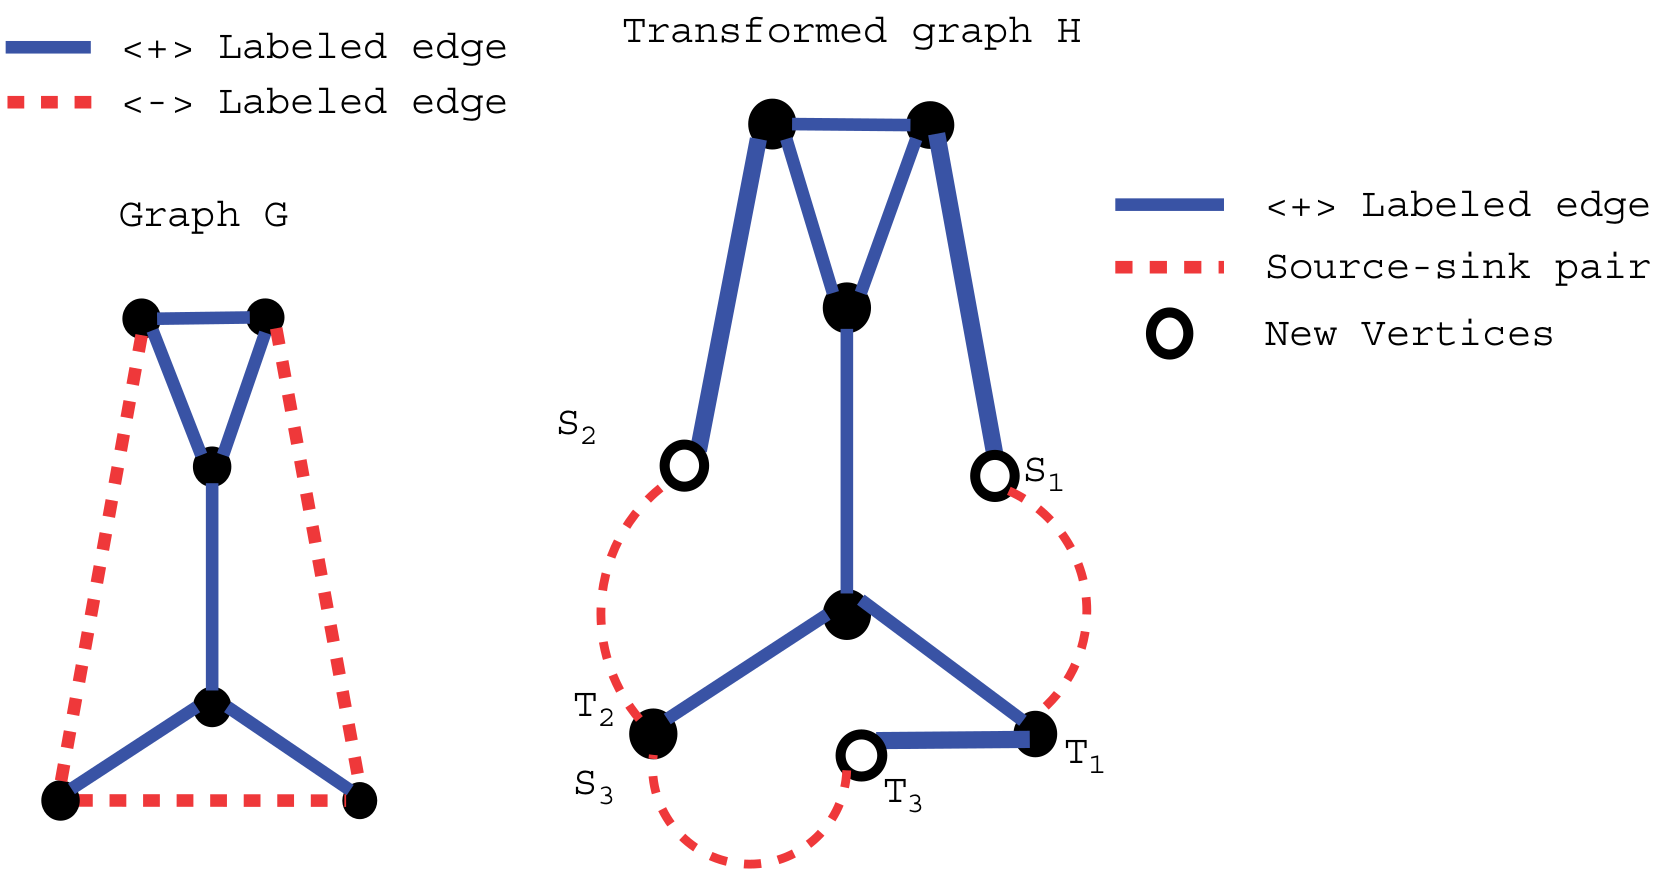
\includegraphics[width=0.8\linewidth]{assets/raw/cc_to_mmc.png}
   \caption{The transformation from \pcc{} on $G$ to \mmc{} on $H$ (reproduced from
   \autocite{Demaine2006}) \label{fig:cc_mmc}}
\end{figure}

If a certain conjecture in computational complexity is true\footnote{Namely, the Unique Game
Conjecture of~\textcite{UGC02}.}, then for every constant $c>0$ it is \NPh{} to approximate \mmc{}
within a factor $c$~\autocite{MulticutHardness06}. On general graphs, the best known approximation factor in $O(\log
k)$~\autocite{RegionGrowing93}, which according to the presented reduction translates to
$O(\log|E^-|)=O(\log n^2)=O(\log n)$. This approximation ratio is achieved by first solving the
relaxation of the integer problem \eqref{eq:mindIP}, where the constraint \eqref{eq:mindInteger} is
replaced by $x_{uv}\in [0,1]$. From now on, we refer to that relaxation as the \emph{canonical
\mind{} LP}. Once this canonical \mind{} LP is solved, we interpret $x_{uv}$ as a distance: the
larger it is and the more we want $u$ and $v$ to be in different clusters. We can then use the
\regionGrow{} method~\autocite{RegionGrowing93}. The idea is to pick a random center $u$ and to add
to $u$'s cluster all the nodes at distance less than $r$ from $u$ before removing that cluster and
repeating the process. $r<\shalf$ is chosen adaptively such that the weight of positive edges
leaving the cluster is less than $c\log(n+1)$ times the fractional weights of the positive edges
inside the cluster.
%\Todo{The full proof can be found in pages 7--9 of
%\href{http://erikdemaine.org/papers/Clustering_TCS/paper.pdf}{this online pdf} but in my opinion, it
%doesn't have much to do with machine learning.}

However, \textcite[Theorem 2]{Charikar2003} note that the LP formulation has a poor integrality gap
when it comes to \maxa{}, thus they turn to a Semi Definite Program. Say that each cluster is
associated with a basis vector, then for each node $u$ in a cluster, we set $a_u$ to be the
corresponding basis vector. If $u$ and $v$ are in the same cluster, we then have $a_u\cdot a_v = 1$
while if they belong to different clusters, $a_u\cdot a_v = 0$. The weighted number of agreements
can then be represented by
\begin{align}
   \label{eq:maxaSDP}
   \text{maximize } & \sum_{(u,v)\in E^+} w_{uv}(a_u\cdot a_v) + \sum_{(u,v)\in E^-} w_{uv}(1-a_u\cdot a_v) \\
   \text{subject to}& \quad a_u\cdot a_u=1 \nonumber\\
   \phantom{subject to}& \quad a_u\cdot a_v\geq 0  \nonumber
\end{align}
After solving the SDP, a clustering can be obtained by a general rounding technique $H_t$: pick $t$
random hyperplanes and divides the nodes in $2^t$ clusters. \Textcite[Theorem 3]{Charikar2003} prove
that taking the best results of $H_2$ and $H_3$ gives in a $0.7664$ approximation on general graph.
This was slightly improved to $0.7666$ by \textcite{Swamy2004} with a different rounding: pick $k$
random unit vectors (called \emph{spokes}) and assign each $a_u$ to the closest spoke.

Combining \mind{} and \maxa{}, \textcite[Section 4]{Charikar2004} give a $\Omega(\frac{1}{\log n})$
approximation of the \textsc{MaxCorr} problem, which is maximizing \eqref{eq:maxa} - \eqref{eq:mind}
and can be formulated as a quadratic programming problem solved in polynomial time.

In complete graphs, \textcite[Section 3]{Charikar2003} also give an improved $4$-approximation to
\mind{}, by rounding the same LP and using a simpler version of \regionGrow{} with fixed radius.
Namely, we pick a ball center $u$ \uar{} with radius \shalf{}: if the average distance of the nodes
in the ball to $u$ is less than $\nicefrac{1}{4}$, the ball forms a cluster, otherwise $\{u\}$ forms
a singleton cluster. We then remove the corresponding nodes from the graph and repeat until all
nodes are clustered.

Not long after, \textcite{CCPivotConf05} came up with a better approximation. To explain it, we
first describe their randomized combinatorial algorithm \ccpivot{}, which gives a $3$-approximation
of \mind{} on complete unweighted graphs (and was later derandomized while preserving its
approximation guarantee~\autocite{derandomCCPivot08}). At each iteration, we pick a node $u$ \uar{}
(called the pivot) and we create a cluster containing $u$ and all its neighbors
linked by a positive edges. On weighted complete graphs, they tweak this algorithm by using the
solution of the canonical LP to obtain different approximation factor depending on the
% \Todo{Comment on those constraints, especially the triangular ones in the context of consensus clustering.}
constraints imposed on the weight. Recall that in the general formulation of the problem, each
edge carries two positive numbers: $w_{u,v}^+$ and $w_{u,v}^-$. If the weights respect the
probability constraints stating that for all edge $(u,v)$ in $E$, $w_{u,v}^+ + w_{u,v}^- = 1$, this
tweaking provide a $2.5$-approximation. Note that unweighted graphs naturally fit into that case, as
each edge is either labeled $+$ or $-$. If the weights
additionally respect the triangular inequality constraints stating that $w_{u,v}^- \leq w_{u,w}^- +
w_{w,v}^-$, this become a $2$-approximation. After solving the canonical LP with additional
probability constraints, when picking a node $u$, each of its neighbors $v$ is added to the cluster
of $u$ with probability $x_{uv}$. \Textcite{Chawla2014} improve these two factors to respectively
$2.06$ and $1.5$ by exploiting the same idea but setting the probability to include each neighbor
$v$ of $u$ in the cluster of $u$ to be $1-f^+(x_{uv})$ if $(u,v)\in E^+$ and $1-f^-(x_{uv})$ if
$(u,v)\in E^-$, with a careful choice of $f^+$ and $f^-$. They also give a derandomized version of
their algorithm in the full version of the paper~\autocite[Theorem 23]{ChawlaArxiv14}.

\begin{table}
   \caption{Best current results on \pcc{} problems. The \enquote{easiest} setting is \maxa{} on
      complete graphs, for it admits PTASs. All others cases are \APXh{}. However, we see that on
      the diagonal (that is \mind{} on complete graphs and \maxa{} on general graphs), there exists
      constant factor approximations. This is not the case for the most \enquote{difficult} problem,
      \mind{} on general graphs. \label{tab:cc_approx}}
   \begin{tabulary}{\textwidth}{lLL}
      \toprule
      $G$      &  \mind{}                                                  & \maxa{}                                 \\
      \midrule
      Complete &  $2.06$ (and $1.5$ if $G$ is weighted and weights obey the triangular inequality) \autocite{Chawla2014}
               & PTAS from \textcite{Bansal2002} and by setting $k=\Omega(1/\epsilon)$ in \autocite{Giotis2006}      \\
      General  &  $O(\log n)$ \autocite{Charikar2003}                      & $0.7666$ \autocite{Swamy2004}           \\
      \bottomrule
   \end{tabulary}
\end{table}

\medskip

This concludes the presentation of the known approximation results on \pcc{}, that we gather in
\autoref{tab:cc_approx}.
To summarize, except for maximizing the number of agreements on a complete graphs, we cannot hope
for exact solutions for the other problems in the worst case, since they are \APXh{}. Moreover, even
constant factor approximation are ruled out for \mind{} on general graphs, as showed by the
equivalence with \mmc{}.
Currently there are three main approaches to approximate \mind{}. On a general graph,
one first solve the canonical LP, and use the \regionGrow{} method to round the fractional solution,
resulting in an $O(\log n)$ approximation. On complete graphs, the simplest solution is the
\ccpivot{} algorithm, that grows clusters out of randomly selected pivots, in a way reminiscent of
the proof of \autoref{thm:weakbal-consistent}. The approximation factor of this general idea can be
improved by interpreting the fractional solution of the linear program as probability to be included
in the pivot's cluster. The cost of solving linear programs with so many variables and constraints
being prohibitive, real world general graphs requires to move from methods with guarantees to more
heuristic approaches we describe next. Before that, we make two remarks. The first one regards a
line of work improving scalability of these approximations by presenting distributed solutions. The
second one is concerned with the case where the number of clusters is set beforehand, and proves
that the problem becomes easier.

\begin{aside}
% \marginpars{maybe I could adapt the proof of lemma 1 to prove the number of rounds of \gtx{},
% although this is quite probabilist.}
To handle the massive size of some large real world dataset, parallelizing existing algorithms is a
natural approach. Due to its simplicity and approximation guarantee, \ccpivot{} has been adapted
three times for that purpose. First, \textcite{Chierichetti2014} describe how to uniformly sample
several pivots in the same round, remove pivots that are adjacent through positive edges and then
grow the corresponding clusters with potential conflicts solved according to the node order in a
global permutation drawn at the beginning of the algorithm. On general graphs, this requires $O(\log
n\diam(G))$ rounds, which on complete graphs reduces to $O(\log n)$.
Furthermore, this almost preserves the approximation factor, which is
$3+\frac{14\epsilon}{1-7\epsilon}$, where $\epsilon$ is a parameter smaller than $1$. Finally, this
allows to experimentally cluster graphs with millions of nodes and billions of edges. Second,
\textcite{ParallelCCNIPS15} describe an equivalent version of \ccpivot{} where a permutation $\pi$
of the nodes is drawn at the start of the algorithm and the pivots are chosen sequentially in the
order of $\pi$. The exact same partition can be obtained when several pivots are chosen at the same
time by different threads as long as they respect two concurrency rules: (i) two nodes $u$ and $v$
can become pivot at the same time if they are not connected with a positive edge, otherwise only the
one with the smallest index in $\pi$ becomes pivot; (ii) if $w$ is a positive neighbor of two pivots
$u$ and $v$, it is affected to the cluster of the pivot with the smallest index in $\pi$. Enforcing
these rules preserves the factor $3$ approximation and the algorithms terminate after $O(\log
n\diam(G))$ rounds. The authors also present a version where each round is faster as it does not
enforce rule (i). However, this weaken the approximation guarantee to $(3 + \epsilon)OPT +
O(\epsilon n\log^2 n)$. In practice, the solution is very close the one of \ccpivot{}, although it
degrades as the number of threads increases.

The number of rounds preserving the $3$-approximation
is lowered to $O(\log\log n)$ by \textcite{Ahn2015}. They also present results obtained in a single
pass, which corresponds to the streaming model: the algorithm receives the edges of $G$ one by one
and upon seeing the last one outputs its result. The additional constraint is that this algorithm
can only use $O(n\polylog n)$ space. In this setting, the authors show a polynomial time
$(1-\epsilon)$-approximation of \maxa{} if the weights are bounded (and $0.766(1-\epsilon)$ if the
weights are arbitrary); and an $O(\log |E^-|)$ approximation of \mind{} in polynomial time with arbitrary
weights. This is done by combining graph sketching and a method to solve convex programs in a space
efficient manner.

\Textcite{Bonchi2013} suggest a different paradigm to solve \pcc{}, that can be applied in a
distributed setting to obtain a scalable approach. Namely, given a node $u$, they want to output a
globally consistent cluster index $\cluster(u)$ while making at most $t$ queries to a sign oracle.
Here $t$ is a parameter that depends on the quality of clustering produced but not on the size of
the graph. And because this procedure is local to each node, it can be run in parallel. Finally, one
can get a full clustering by computing $\cluster(u)$ for all the nodes in the graph. Despite the
problem being apparently more challenging, they obtain approximation factors that are close to the
best known (which in this model would make $\Omega(n^2)$ total queries). More precisely, they use
two techniques.
The first one is inspired by \ccpivot{}. It starts by finding a good set of pivots, seeing the
problem as finding a maximal independent set on a sampled part of the positive graph. Then, for a
given node, it finds the closest such pivot or creates a singleton. Given a quality parameter
$\epsilon\in(0,1)$, it yields a $4\cdot OPT + \epsilon n^2$ approximation of \mind{} requiring
$O(\frac{n}{\epsilon})$ time and queries~\autocite[Theorem 3.3]{Bonchi2013}.
Roughly stated, the second one relies on an existing low-rank approximation of the adjacency matrix,
that partition the graph into similar sized classes such that edges between those classes behave as
in a random graph. This initial partition is \enquote{coarsened} into a good clustering by
considering all possible ways of assigning classes to clusters. It gives an $OPT + \epsilon n^2$
additive approximation  for \mind{} that runs in time $n \cdot poly(\nicefrac{1}{\epsilon}) +
2^{poly(\nicefrac{1}{\epsilon})}$ \autocite[Corollary 3.7]{Bonchi2013}.
\end{aside}

\begin{aside}
As mentioned earlier, not having to set the number of clusters is an
attractive feature of the \pcc{} problem, but in some cases we may want to use prior knowledge.  The
problem was studied by \textcite{Giotis2006} on general graphs and we compile their results in
\autoref{tab:cc_fixed}. On complete unweighted graphs and with $K$ being the number of clusters, they
provide PTASs for \maxa{}$[K]$ running in $nk^{O(\epsilon^{-3}\log(\frac{K}{\epsilon}))}$ time and for
\mind{}$[K]$ running in $n^{O\left(\epsilon^{-2} 9^K\right)}\log(n)$ time. The latter was improved by
\textcite{LinearMinPTAS09}, with a PTAS running in $n^2 2^{O\left(\epsilon^{-3}K^6\log d\right)}$
and that can handle weighted graphs. For $K=2$, \mind$[2]$ admits a faster local search method with a
factor $2$ approximation~\autocite{Coleman2008}.
For complete weighted graph, \textcite{WeightedMaxAPTAS08} provide a PTAS for
\maxa{}$[K]$ under the condition that the ratio between the largest and smallest weights is bounded by a
constant.
\begin{center}
   \captionsetup{font=small}
   \captionof{table}{\label{tab:cc_fixed} Approximation results for \pcc{} on general graphs with $K$
   clusters}
   % 187mm - 3em = https://tex.stackexchange.com/a/8263
   \begin{tabulary}{177mm}{lLL}
      \toprule
      $K$	 & $2$ & $\geq 3$ \\
      \midrule
      \maxa{} & $0.878$ (improved to $0.884$ by \autocite{Mitra2009}) & $0.7666$
      \autocite{Swamy2004} (and it can be proved that this creates at most $6$ clusters) \\
      \mind{} & $O(\sqrt{\log n})$ as it reduces to Min 2CNF Deletion for which \textcite{min2CNF05}
      give such an approximation &
      this can be reduced from $K$-coloring, which for any $\epsilon > 0$ is \NPc{} to approximate
      within $n^{1-\epsilon}$ \autocite{InnaproxChroma07} \\
      \bottomrule
   \end{tabulary}
\end{center}
\end{aside}


\subsubsection{Heuristics}
\label{ssub:cc_heuristics}

While all the methods we discuss so far
are either exact or come with some approximation guarantees, practitioners have also develop
approaches that are designed to efficiently reach a solution that is satisfactory enough for the
application at hand.
% \url{http://ieeexplore.ieee.org/document/7321476}

\paragraph{Greedy methods}
\label{par:cc_greedy}
Several of such methods fall into the greedy framework.
For instance, while studying small scale signed social networks,
\textcite{Early96} describe the following procedure. Start with a random initial $k$ clustering of
the graphs and for $T$ steps, sample randomly $P$ neighboring partitions, compute their number of
disagreements and move the one with the least disagreements. Neighboring partitions are obtained
either by moving one node from cluster to another or by exchanging a pair of nodes between two
clusters. The overall complexity is $O(nTP)$. This is quite similar to the \emph{Best One Element
Move} described in~\autocite{Gionis2007}, except that there the exchange operation is replaced by moving
one node to its own singleton cluster. The \emph{Cluster Affinity Search Technique}
algorithm~\autocite{Ben-Dor99} instead grows clusters one by one by maintaining for the current
cluster the affinity of all nodes, which is the sum of the weights between that node and the nodes in
the cluster. Nodes above a certain threshold are added to the current cluster and nodes below the
threshold are removed, with the affinity to the current cluster being recomputed after each addition
or deletion.

After defining the net weight of an edge to be $w^\pm_{uv} = w^+_{uv} - w^-_{uv}$,
\textcite{Elsner2009} describe three folklore heuristics that start with empty clusters and add node
one by one: \enquote{The \textsc{Best} algorithm adds each node $u$ to the cluster with the
strongest $w^\pm$ connecting to $u$, or to a new singleton if none of the $w^\pm$ are positive.
The \textsc{First} algorithm adds each node $u$ to the cluster containing the most recently
considered node $v$ with $w^\pm_{uv} > 0$. The \textsc{Vote} algorithm adds each node to the cluster
that minimizes the \pcc{} objective, \ie{} to the cluster maximizing the total net weight
or to a singleton if no total is positive.} Empirically, \textsc{Vote} turns out to be the best.
Among other related heuristics, \textcite{mergingHeuristics14} describe the random maximum merging
algorithm, that starts with singleton clusters and keep merging two clusters chosen at random among
those whose merge would result in the maximum improvement of the score function. This runs in
$O(n^2\log n)$, and empirically results in fewer disagreements than \ccpivot{}.
Building upon their previous GRASP work~\autocite{GRASP13}, an iterated local search (ILS) heuristic is
presented in~\autocites{Levorato2015}{Levorato2017}. Each iteration of this algorithm starts by
greedily build a clustering in fashion similar to \textsc{Vote}, albeit with more randomness in the
node ordering. This clustering is locally improved by moving blocks of $r\in\{1,2\}$ nodes from one
cluster to another as long as the number of disagreements decreases, a phase called neighborhood
descent. The algorithm then enters an inner loop where the current clustering is perturbed by $t$
random one-node-moves and updated if a subsequent neighborhood descent can improve it compared with
before the perturbation. The authors note that both the outer loop and the neighborhood descent can
be run in parallel, which allow them to process a \np{10000} nodes graph on 10 cores in around 700
seconds. \Textcite{heuristicCE16} show how to use ILS to generate initial solutions of the Cluster
Editing problem that are then fed to an integer program.
% This local search followed by random perturbation is reminiscent of genetic algorithms, and such an
% approach is sketched in~\autocite{GeneticCC08}.\footnote{but that's a terrible paper!}
Instead of
moving nodes, \textcite{restoreNeighborhood13} starts from the observation that in a balanced
graph, $G^+$ is a disjoint union of cliques in which all the nodes of a given cluster share the shame
neighbors. Their algorithm is initialized with the set $E_s^+$ of edges where $w^+_{uv} > w^-_{uv}$,
and repeatedly samples an edge $(u,v)$ from $E_s^+$ before trying to make the neighborhoods of $u$
and $v$ coincide by adding or removing edges in $E_s^+$.  Yet another idea is to modify the
canonical LP to replace the binary variable $x_{uv}$ by a $k$ clusters indicator matrix
$L\in\Rbb^{k\times n}$ where $L_{iu}$ is $1$ is $u\in C_i$ and $-1$
otherwise~\autocite{AltOptimLP13}. Indeed, $x_{u\cdot} \equiv L_{\cluster(u)\cdot}$, where $\cluster$
is the cluster assignment. By relaxing the integer constraints on $L$, it is possible to do
alternate optimization on $L$ and $\cluster$.

\paragraph{Physics inspired energy methods}
\label{par:cc_physics}

Here we describe a physics particle model that can readily be adapted to model \pcc{} and provide
additional heuristic methods.
The Potts model~\autocite{PottsSurvey82} describes a general model of \emph{spins} organized in a
lattice and being in one of $k$ possible states. A spin $u$ interacts with each of its neighbors $v$
through a coupling $J_{uv}$. The energy of this system, called the Hamiltonian, is defined by
$\mathcal{H}(\bm{\sigma}) = -\sum_{u,v} J_{uv} \delta(\sigma_u, \sigma_v)$ where $\bm{\sigma}$ is
the spin configuration (that is, $\sigma_u \in \{1,\ldots,k\}\,\forall u$) and $\delta(\sigma_u,
\sigma_v)$ is equal to one if $u$ and $v$ are in the same state and zero otherwise. It is a general
principle of physics that isolated systems tend to minimize their energy, which in this case amounts
to finding a spin configuration minimizing the Hamiltonian. Viewing the spins as nodes of a graph,
the couplings as the graph weighted edges and the $k$ possible states as clusters, it is quite
natural to formulate the clustering problem as a Hamiltonian minimization
problem~\autocite{CommunityPhysics06}.

Letting $A$ be the matrix such that $A_{uv} = w_{uv}^+ -
w_{uv}^-$ on a general directed graph, \textcite{Traag2009} reward positive and absent negative
links within cluster and penalize negative and absent positive links across clusters to come up with
the following Hamiltonian: $\mathcal{H}(\bm{\sigma}) = -\sum_{u,v} \left(A_{uv}-(\gamma^+p^+_{uv} -
\gamma^-p^-_{uv})\right) \delta(\sigma_u, \sigma_v)$ where $\gamma^+$ and $\gamma^-$ are user
parameters and $p^\pm_{uv}$ are null model probabilities, which are equal to $p^\pm_{uv} =
\frac{|E^\pm|}{|V|(|V|-1)}$, or $p^\pm_{uv}=\frac{\dout^\pm(u) \din^\pm(v)}{|E^\pm|}$ in the degree
corrected model. They note that setting $\gamma^+ = 0 = \gamma^-$ make minimizing the Hamiltonian
equivalent to the \mind{} problem, which they do by simulated
annealing~\autocite{SimulatedAnnealing83}. The idea is to start from a random partition, and jump to
another partition by moving a single node from one cluster to another. Such moves are made with a
probability proportional to how each move reduces the Hamiltonian and as the procedure goes on, large
jumps are made less and less probable by reducing a parameter called the temperature.
One advantage of this energy formulation is that it requires only one variable per node instead of
one variable per edge as in the case of the linear program.

In the case of $2$-\pcc{}, \textcite{Facchetti2011isingmodel} rewrite the Hamiltonian as
$\mathcal{H}(\bm{\sigma}) = -\frac{1}{2}\bm{\sigma}^T A \bm{\sigma} = -\frac{1}{2}\bm{1}^TT_\sigma A
T_\sigma\bm{1}$. There $T_\sigma = diag(\bm{\sigma})$ (where $\bm{\sigma} \in \{0,1\}^n$) is the
outcome of a local search algorithm such that $A_\sigma = T_\sigma A T_\sigma$ has the same number
of disagreements as $A$ but the smallest number of negative edges. This is called a gauge
transformation in the spin glass literature and the benefit of that heuristic is that it scales
gracefully to large graphs.
\Textcite{Bagon2011} also write the \maxa{} objective as a Potts model, and show that it can be
interpreted as the log posterior of a partition matrix under a simple generative model and as a
pair-wise conditional random field energy without unary terms. This allows them to adapt existing
discrete energy optimization algorithms in order to cope with the following three challenges of the
\pcc{} energy: \enquote{(i) the energy is non sub-modular, (ii) the number of clusters is not known
in advance, and (iii) there is no unary term}. Doing so, they are able to handle large problems with
more than 100K nodes.  Also adopting an energy minimization approach, \textcite{Kappes2016} assign a
probability to each cut of a signed graph proportional to the exponential of the number of
disagreements of that cut. They also develop efficient cut sampling methods. Several of these
methods have recently been evaluated empirically by \textcite{energyCCBench17}.

% something about local minima when defining another energy function, and how it is achieved by a
% dynamic model but to be honest it has little to do with clustering {Marvel2009landscape}
% does it have something to do with phase transition
% Kappes2016 \enquote{Furthermore, due to the lack of an external field (unary terms), any permutation of an
% optimal assignment results in another optimal labeling.}
% like an ICML'17 paper that touches something very related (multicut) and gives recent applications in
% vision https://arxiv.org/abs/1503.03791 represents a cut by the set of interclusters edges


\subsubsection{Active and online settings}

Except for the local algorithms of \textcite{Bonchi2013}, all works presented so far considered the
batch case of \pcc{}, where the whole graph and all the signs are available at all time and with no
cost. This might not always be the case, for instance if the graph is too large to fit in memory or
if the edge labels are given by an expensive external procedure.

% \emph{Still have to write this part. Is there a link between mistake bound and approximation
% ratio?} say I have a binary classifier that perfectly predict sign wrt to the optimal clustering
% C* those below are more concerned with sign prediction than clustering per se Beside batch
% setting, one can also consider active \autocites{Cesa-Bianchi2012b}{Cesa-Bianchi2012a} and online
% \autocite{Gentile2013} framework.
% \enquote{the work of Cesa-Bianchi et al. [CBGV+12] that take a learning-theoretic perspective on the
% problem of predicting signs. They consider three types of models: batch, online, and active
% learning, and provide theoretical bounds for prediction mistakes for each setting. They use the
% correlation clustering objective as their learning bias, and they show that the risk of the
% empirical risk minimizer is controlled by the correlation clustering objective.}

Case in point, in the context of entity resolution, \textcite{activeCoref07} consider the \pcc{}
problem where, by querying an oracle, one can either reduce the uncertainty about one edge weight or
add an extra node with edges connecting it to existing nodes. However, this requires web queries
that are resource bounded and thus yields an active setting learning problem, where one has to
choose the most informative
queries given a budget. A formal definition is given in~\autocite{queryMoreEdgeCC07} and in
practice, after finding an initially good partition, they select in each cluster a node to be its
centroid, and query the edges connecting the centroid as ordered by an entropy-based criterion.
In the case the oracle answering the queries is consistent, then there exists an information
theoretic bound on the number of queries needed to recover the clusters, and an algorithm matching
that bound up to a $O(\log n)$ factor~\autocite{perfectActiveLong17}.
\textcite[Section 5]{Ailon2014} present another active algorithm that solves \mind$[k]$ with a
linear number of queries but an exponential running time in $n$.  In a noisy setting,
\textcite{Mitzenmacher2016} assume there is a planted $k$-partition and that we have access to an
oracle that for $u,v\in V^2$ returns $\cluster(u) - \cluster(v) \mod k$ with probability $1-p$ and a
noisy $\cluster(u) - \cluster(v) \pm 1 \mod k$ otherwise. For $k=2$, this is exactly $2$-\pcc{},
whereas for $k>2$, the oracle gives more information than simply the sign of the path from $u$ to
$v$. Whenever
$p < \shalf$, they show that $O(n^{1+\frac{1}{\log\log n}}\log n)$ queries are enough are to recover
the planted partition in polynomial time and with high probability. Those queries are actually
random (\ie{} non-adaptive), and the clusters are found by looking at almost edge-disjoint path
between all pairs of nodes.
% this was improved in https://arxiv.org/abs/1709.07308

In the online setting, \textcite{greedyOnline10} give a greedy algorithm that upon node arrival creates a
singleton cluster and then merge all pairs of clusters for which it increases the total number of
agreements. For \mind{}, this is $O(n)$-competitive algorithm and they show such ratio is optimal by
exhibiting an instance\footnote{Namely, two positive cliques $A$ and $B$ joined by positive edges except
between $a\in A$ and $\{b_1,\ldots, b_k\}\in B$. Those nodes are given first and thus form a cluster,
which yields at least one disagreement every time one the $n-(k+1)$ remaining nodes is added.} on
which any strategy ends up with $n - k$ disagreements whereas optimal cost is $k$. On the \maxa{}
side, this greedy strategy result in a $\shalf$-competitive algorithm. If it is randomly mixed with a
\textsc{Dense} variation, it increases to $\shalf+\eta$, still far from the demonstrated $0.834$ upper
bound.
% when the graph is given node by node,
% \url{https://link.springer.com/chapter/10.1007/978-3-319-18173-8_7} show to cluster it in static
% clique, so it sounds related to cluster editing, except their objective is to maximize the
% fraction of edge in cliques (ie avoid small cluster)

\bigskip

This state of the art depicts a nuanced landscape for the \pcc{} problem. On one hand, minimizing
the disagreements is difficult, although it is the most natural way given our bias. On the other
hand, it can be solved with approximation guarantees, at least in theory. Indeed, the best methods
requires solving linear programs with $m$ variables and up to $O(n^3)$ constraints, which results in
a high complexity of $O(m^{4.5})$~\autocite[Section 7.2]{LPBook07}. Fortunately, we can obtain
reasonable solutions in practice, thanks to efficient heuristics (using the output of \ccpivot{} as
initialization for instance). Furthermore, instances obeying our bias can be solved more easily and
almost exactly. We next present settings where instances are indeed close to our bias.
Before that, we remark that whereas \ccpivot{} is often used on general graphs in practice by
assuming the missing edges are negative, doing so does not preserve its approximation guarantee.
\begin{marginfigure}
  \centering
  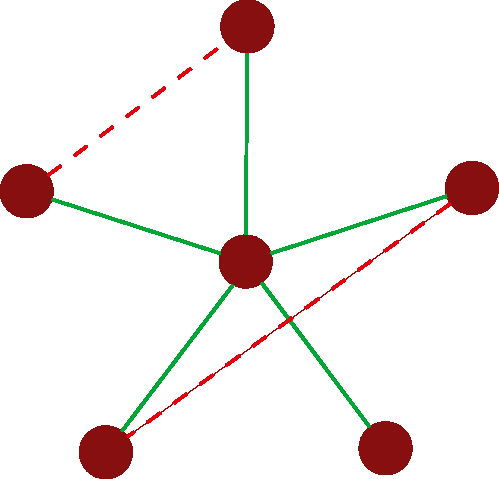
\includegraphics[width=\linewidth]{assets/raw/pivotstar.pdf}
  \caption{A positive star with few negative edges}
  \label{fig:cc_star_pivot}
\end{marginfigure}

\begin{aside}
   Consider the graph $G$ showed in \autoref{fig:cc_star_pivot}. Assume there are $n$ nodes
   connected positively to the center of the star, and $k<n-1$ negative edges between the peripheral
   nodes. We define $G'$ as the complete graph obtained from $G$ by setting all missing edges to be
   negative. On $G'$, the optimal solution is to have a cluster with the center of the star and one
   peripheral node, while others peripheral nodes are put in singleton clusters. This creates $n-1$
   positive disagreements. When running \ccpivot{} on $G'$, if the first pivot is a peripheral node,
   this is the solution we obtain. Otherwise, with probability $\nicefrac{1}{n}$, the center of the
   star is chosen as pivot, creating a single big cluster that incurs $(\shalf)(n-1)(n-2)$ negative
   disagreements. In expectation, \ccpivot{} thus achieves \[
   \frac{1}{n}\left(\frac{(n-1)(n-2)}{2}+(n-1)^2\right)=\frac{3n-4}{2n}(n-1)\sim \frac{3}{2}n \]
   disagreements, which is roughly a $\nicefrac{3}{2}$-approximation as $n$ grows larger.

   Now let us get back to the original $G$. Here the optimal solution is to have a single big
   cluster, which incurs $k$ negative disagreements. With the same reasoning as before, the expected
   number of disagreements of \ccpivot{} is now $\frac{1}{n}\left(k+(n-1)^2\right)$. If for
   instance $k=\floor{\sqrt{n}}$ (as in \autoref{fig:cc_star_pivot}), then the previous expression
   is equivalent to $n$ as $n$ tends to infinity. \ccpivot{} is thus $\sqrt{n}$ worst in expectation
   than the optimal when run on this general graph.
\end{aside}
